% Divergencia: flujo v_z por las caras inferior y superior del cubo (libro fig. 2.7)
\documentclass[border=5pt]{standalone}
\usepackage{tikz}
\usetikzlibrary{arrows.meta, calc}
\begin{document}
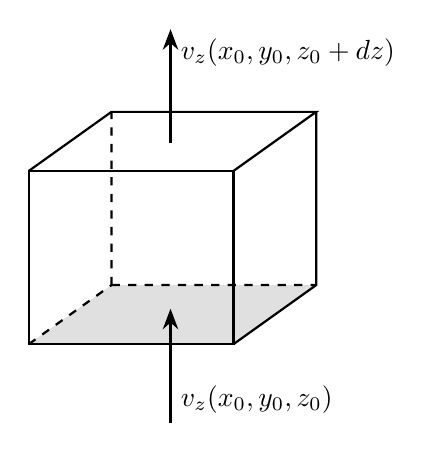
\begin{tikzpicture}[>={Stealth[length=2.6mm]}, line width=0.8pt]
  \coordinate (A) at (0,0);
  \coordinate (B) at (2.6,0);
  \coordinate (C) at (2.6,2.2);
  \coordinate (D) at (0,2.2);
  \coordinate (A2) at (1.05,0.75);
  \coordinate (B2) at (3.65,0.75);
  \coordinate (C2) at (3.65,2.95);
  \coordinate (D2) at (1.05,2.95);
  % cara inferior sombreada (A,B,B2,A2)
  \fill[black!12] (A)--(B)--(B2)--(A2)--cycle;
  \draw[dashed] (A2)--(B2) (A2)--(D2) (A)--(A2);
  \draw (A)--(B)--(C)--(D)--cycle;
  \draw (D)--(D2)--(C2)--(C) (B)--(B2)--(C2);
  % flujo entrante por la cara inferior y saliente por la superior
  \draw[->, line width=1.1pt] (1.8,-1.0)--(1.8,0.45);
  \node[right] at (1.8,-0.7){$v_z(x_0,y_0,z_0)$};
  \draw[->, line width=1.1pt] (1.8,2.55)--(1.8,4.0);
  \node[right] at (1.8,3.7){$v_z(x_0,y_0,z_0+dz)$};
\end{tikzpicture}
\end{document}
